
\chapter{System design}
\section{System overview} \label{sec:system}
\begin{comment}Here you insert a block diagram of your voltage regulationa nd signal conditioning system. 
Try to explain \textbf{what} configiation you chose and \textbf{why}. 
There is no need to specify the capacitor and resistor values here, but you want to capture the higher-level functional arrangement you have opted for. The diagram ties together the other chapters in this report and helps the reader understand how you have connected the different funtional blocks together to produce the outputs. For example, a block could be ``Differential amplifier'' or ``level shifting op-amp'' or ``Low-pass filter'' or ``Linear regulator'' and the like. 
Please use a drawing application, such as draw.io, MS Visio, or Power Point and export it as a PDF, so it looks good. If you feel brave, draw them in \LaTeX using Inkscape/\texttt{TikZ}.
Fig.\ \ref{fig:system_diagram} is a bad example that is completely irrelevant and just holds space for your beautiful system diagram.
\end{comment}

The system diagram of the voltage regulation and signal conditioning system can be seen in Fig.\ \ref{fig:system_diagram}, as well as the definitions of the signal lines.\newline
 A linear voltage regulator is chosen to supply the circuit with power. Though inefficient in comparison to a switch mode regulator, the motivation of this design choice is further explained in a later chapter. The differential amplifier was chosen in order to minimise the need for more than one op-amp for signal conditioning. A summing amplifier could just as well be used, whoever it would require two or more op-amps.  To ensure that the \SI{5}{VDC} source is not affected by the amplifier, a buffer is used in between the voltage regulator and the differential amplifier. This circuit does not allow the use of negative voltages at the negative power supply pin, which means the amplifier can only swing  between $5V$ and ground. A virtual ground offset of $2.5V$ is therefore used to center the temperature response. The last conditioning o the signal is a Low Pass Filter that suppresses signals of \SI{50}{\Hz} to \SI{50}{\milli\V} inaccuracy In order to meet the total current requirement, all if not most resistors in the circuit network will be in the order of \SI{}{\kilo\Omega} to minimise current flow.
 \newline
\begin{figure}
    \centering
    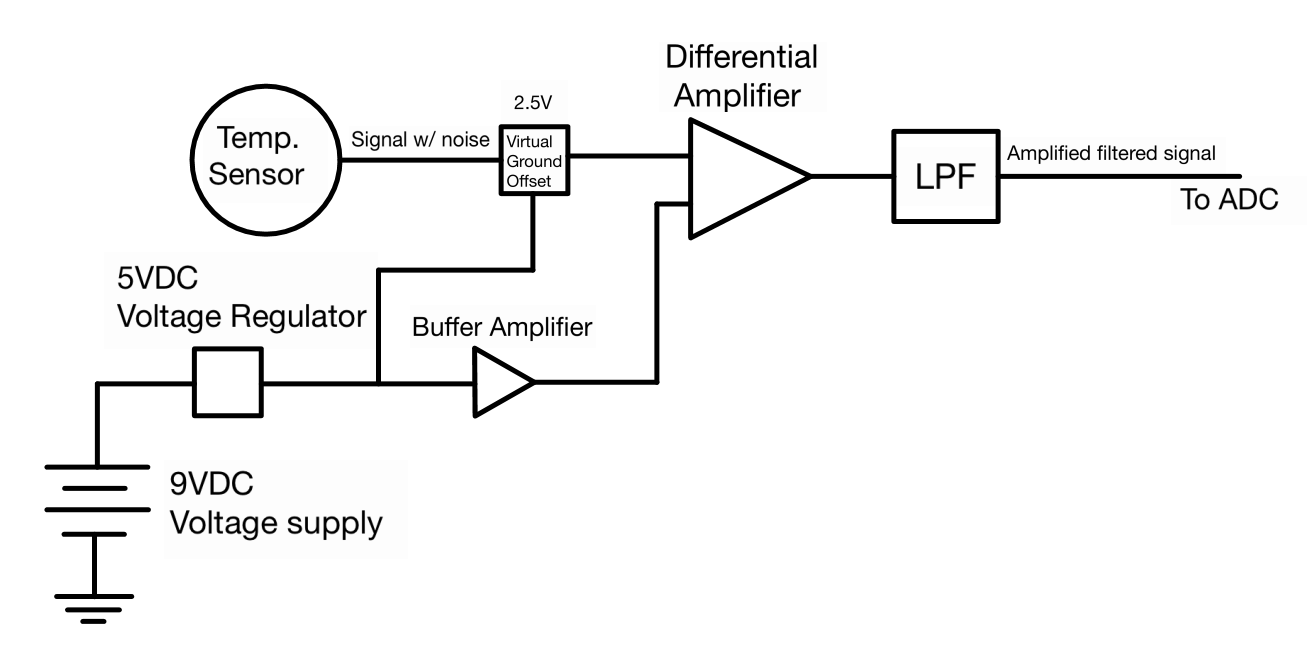
\includegraphics[width = 0.8\linewidth]{Figures/Pictures/SystemDiagram.png}
    \caption{System diagram}
    \label{fig:system_diagram}
\end{figure}

\vfill









